\documentclass{article}
\usepackage[utf8]{inputenc}
\usepackage{pdfpages} 
\usepackage[czech]{babel}
\usepackage{amsfonts,amsmath}

\usepackage{natbib}
%\bibliographystyle{abbrvnat}
\bibliographystyle{plainnat}
\setcitestyle{authoryear}

\usepackage[colorlinks=true]{hyperref}

\title{Koncept predikce bezpečnostních indikátorů EDZ}
\author{Jan Březina}
\date{leden 2020}

\def\prtl{\partial}
\def\vc#1{\mathbf{\boldsymbol{#1}}}     % vector
\def\tn#1{\boldsymbol{#1}}
\def\todo#1{{TODO:\color{red}#1}}

\begin{document}

\maketitle


\section{Úvod}
Bezpečnost plánovaného hlubinného úložiště vysoce aktivních jaderných odpadů je zajištěna 
jednak inženýrskými bariérami (obalový soubor, bentonitové utěsnění) a dále geologickou bariérou 
– horninovým masivem. Pro konstrukci úložiště jsou v horninách raženy chodby, přičemž dochází 
k narušení okolní horniny na vnitřním okraji geologické bariéry a vzniká tzv. zóna poškození 
(EDZ - excavation damage zone). 
Zejména v krystalických (křehkých) horninách vzniká síť nových (mikro) puklin, která zvyšuje 
hydraulickou vodivost a může tvořit preferenční cesty podél 
chodeb úložiště a dále skrze případné geologické poruchy k povrchu.
Cílem projektu Endorse je vytvoření metodiky pro predikci odvozených veličin charakterizujících 
bezpečnost EDZ, tzv. indikátorů bezpečnostních funkcí (dále jen jako indikátory bezpečnosti), 
a to na základě cenově dostupných geofyzikálních měření. Výsledkem projektu má být matematický 
model realizovaný pomocí specializovaného výpočetního software a metodika pro posouzení 
bezpečnosti EDZ v dílčích částech budovaného úložiště.
Tento pracovní dokument popisuje předběžný návrh této metodiky a přesněji definuje indikátory 
bezpečnosti. Dále jsou vytipovány hlavní otevřené problémy, na které se musí projekt zaměřit a je 
shrnuta základní rešerše zdrojů k dané problematice. 

Koncepce metodiky a matematického modelu pro predikci indikátorů bezpečnosti EDZ  vychází z předpokládaného průběhu prací při budování a provozování úložiště:
\begin{enumerate}
    \item Z hlavního překopu je proveden horizontální průzkumný vrt v ose budoucí úložné chodby (vertikální ukládání) resp. úložného vrtu (horizontální ukládání).
    \item Na průzkumném vrtu je provedena sada geofyzikálních měření, např:
    \begin{itemize}
        \item optická a ultrazvuková karotáž - identifikace protnutých geologických poruch;
        \item ERT vůči sousední paralelní chodbě;
        \item seismika vůči sousední paralelní chodbě;
        \item tlakové zkoušky v různých úsecích vrtu.
    \end{itemize}
    \item \label{item_model1}
    S pomocí software, jenž bude výsledkem projektu, je proveden výpočet indikátorů bezpečnosti.
    \item Na základě výsledků predikce indikátorů a dle expertního posouzení se určí počet bezpečných úložných pozic a rozhodne se, zda a v jakém rozsahu bude provedena ražba  konkrétního úložného vrtu.
    \item Po vyražení jsou získána další data na povrchu nově vyražených prostor: optické mapování, geofyzikální radar, ultrazvuk, ERT, seismika pro charakterizaci skutečné EDZ a 
          upřesnění makroskopických poruch.
    \item Data jsou použita k \uv{učení modelu} ve smyslu vylepšení priorů Bayesovských modelů. 
    \item \label{item_model2}
    Na základě upřesněného modelu a dle expertního posouzení se určí, které úložné pozice budou skutečně použity.
\end{enumerate}

Komplexní model pro predikci indikátorů bezpečnosti (viz. bod \ref{item_model1} a bod \ref{item_model2}) je složen ze tří navazujících částí: 
    \begin{enumerate}
    \item Na základě kombinované inverzní úlohy jsou odhadnuty hydraulické a mechanické
     parametry \uv{neporušené horniny} a polohy známých geologických poruch a rozhraní. Tyto veličiny jsou identifikovány ve smyslu Bayesovské inverze jako posteriorní rozdělení.
    \item Pomocí modelu EDZ jsou predikovány vlastnosti EDZ na základě vlastností neporušené horniny.
    \item Pomocí modelu transportu jsou predikovány indikátory bezpečnosti pro jednotlivé úložné pozice.
    \end{enumerate}
Podobně je strukturován i tento dokument, ale postupuje naopak od definice indikátorů bezpečnosti k získávání dat z měření: V části \ref{sec:transport} je popsána koncepce modelu transportu v měřítku úložné chodby a jsou definovány indikátory bezpečnosti jakožto veličiny odvozené z tohoto modelu. Je provedena elementární rozvaha ohledně neurčitosti vstupních parametrů modelu. Dále je v části
\ref{sec:model_EDZ} popsána koncepce modelu vlastností EDZ v měřítku jednoho úložného místa. 
V kapitole \ref{sec:parameters} jsou popsána možná měření vhodná pro identifikaci 
parametrů modelů. Pro vybraná měření jsou popsány inverzní úlohy pro identifikaci těchto parametrů.


\section{Model transportu a definice indikátorů bezpečnosti}
\label{sec:transport}
\subsection{Geometrie}
Cílem modelu je postihnout šíření kontaminace z daných úložných pozic do preferenčních cest širší geologické bariéry. Pro zjednodušení uvažujeme pouze systém horizontálního ukládání, viz.  pracovní dokument SÚRAO \uv{Profily jednotlivých chodeb HÚ}, příloha A. Geometrie transportního modelu bude zahrnovat úložné pozice v jednoho úložného vrtu o předpokládané délce 300 metrů. Dále jsou uvažovány  struktury, které mohou představovat preferenční cesty do výrazných geologických poruch v okolí úložiště. Konkrétně jsou do geometrie modelu zahrnuty bezprostředně sousedící úložné vrty a hlavní překop. Vzdálenější vrty budou případně uvažovány pouze jako kontinuum s efektivní anizotropní hydraulickou vodivostí zahrnující vliv EDZ. 
Ještě nevyražené chodby jsou konzervativně předpokládány v plné délce. Do geometrie budou zahrnuty též významné známé pukliny (geologické poruchy) a dále náhodné neznámé pukliny dle předpokládaných rozdělení puklin.

% TODO: zahrnout do plánu prací úpravu algoritmů pro generování puklin aby zahrnuly známé pukliny.


\subsection{Vliv EDZ}
Přímým vlivem ražby a díky změně mechanického napětí v  okolí důlního díla dochází v nejbližším okolí stěn díla k mechanickému poškození horniny a zvýšení hydraulické vodivosti. Tuto oblast nazýváme zóna poškození (excavation damage zone - EDZ). Míra poškození není přesně ohraničena, ale poměrně rychle klesá se vzdáleností od stěny díla. Její efektivní dosah je v řádu centimetrů v případě mechanické ražby (tunel boring machine - TBM) respektive v řádu decimetrů v případě klasické ražby s odstřelem (drill and blast). Na rozdíl od volných chodeb, které mohou být utěsněný různými inženýrskými postupy (bentonit, beton), není možné EDZ v rozashu celého úložiště efektivně utěsnit a představuje tak hlavní transportní cestu mezi zdrojem kontaminace a případnými geologickými poruchami protínající chodby díla.

Kromě zóny mechanického poškození horniny dochází vlivem odčerpávání podzemní vody ke změně hydraulických poměrů ve větším okolí díla nazývaném zóna ovlivnění (excavation disturbance zone). Díky kontaktu s atmosférou v bezprostředním okolí stěny díla dochází k chemickým změnám, které mohou ovlivnit zejména difúzní a sorpční vlastnosti horniny. Tyto jevy nebudou ve výsledné metodice uvažovány, ale pro výsledné použití je třeba posoudit jejich vliv na výsledky modelu.

EDZ podél chodeb bude zachycena buďto pomocí zjemněné 3d sítě nebo jako porucha pomocí 2D prvků. Ve druhém případě je třeba použít pomocný model pro určení ekvivalentních anisotropních tensorů vodivosti a difúze. Síť plného nebo pomocného modelu musí zachytit prostorovou změnu parametrů 
se vzdáleností od stěny díla. Cílem modelu vzniku EDZ (viz. sekce \ref{model_EDZ}) je určit tenzor hydraulické vodivosti, hodnoty disperzních a difúzních parametrů v závislosti poloze, zejména na vzdálenosti od stěny díla.
Prostor chodeb bude uvažován již po zpětném vyplnění (backfill) bentonitem. Vzhledem k velmi malé vodivost nasyceného bentonitu  bude tato oblast z modelu odstraněna jako nevodivá.

\subsection{Další parametry modelu}
Na uvedené oblasti bude uvažována úloha ustáleného proudění s předepsanou tlakovou výškou na vnější hranici danou regionálním modelem proudění. Pro testování SW v rámci projektu bude použit regionální model z parallelního projektu Geotran. Na stěnách díla bude uvažován nulový tok vody. 
Následně bude řešena úloha difúzního transportu stopovače, t.j. bez sorpce v hornině. Jedná se o nejkonzervativnější model, reálné kontaminanty budou retardovány díky sorpci do matrice. Pro posouzení jedné úložné pozice bude v příslušné části úložného vrtu uvažována okrajová podmínka na stěně díla předepisující tok stopovače jakožto funkci času. Časový průběh bude převzat z modelů zdrojového členu.

% TODO: statistika časového průběhu zdrojového členu
%

\subsection{Indikátory bezpečnosti}
Cílem modelu transportu je predikce indikátorů bezpečnosti. Indikátory jsou veličiny, které nějakým způsobem charakterizují bezpečnost úložiště, zde konkrétně bezpečnost jedné úložné pozice z hlediska možnosti úniku kontaminace na povrch. Označme $c_p(t)$ 
časový průběh maximální koncentrace na okraji výše popsaného modelu transportu pro zdroj kontaminace na úložné pozici $p$. Obvykle se toto maximum bude realizovat někde na průsečíku některé významné pukliny s hranicí modelu
a předpokládáme, že $c_p(t)$ je zanedbatelná pro dostatečně velký čas $t>T$.
Jedním z možných indikátorů bezpečnosti by mohla být maximální koncentrace
\begin{equation}
    I_1(p) = c_p^{max} = \max_{t\in(0, T)} c_p(t).
\end{equation}
Tato veličina však nemusí být vhodná vzhledem k dalším difúzním procesům při transportu geologickou bariérou.
Průběh $c_p(t)$ s krátkým pulzem a velkým $c_p^{max}$ může vést na nižší maximální koncentraci na povrchu než v případě konstantního průběhu $c_p(t)$ s menším  $c_p^{max}$.

Transport skrze geologickou bariéru lze zjednodušeně popsat jednorozměrnou rovnicí advekce difúze:
\begin{equation}
    \label{eq:ad}
    R\partial_t c + v \partial_x c - d \partial^2_x c = - \lambda c,
\end{equation}
kde $c(t,x)$ je koncentrace rozpuštěné látky, $R$ je retardační faktor zahrnující vliv sorpce a difúze do matrice, $v$ je průměrná Darcyovská rychlost, $d$ je difúzní koeficient (zahrnující též disperzi) a $\lambda$
je koeficient rozpadu zahrnující jednak radioaktivní rozpad, zejména však ředění nekontaminovanou vodou. 
Předpokládáme řešení na časovém intervalu  $[0, T)$, s nulovou počáteční podmínku $c(t=0, x) = 0$ a na prostorovém intervalu $[0, L)$ se zadaným 
průběhem koncentrace v počátku $c(t, x=0) = c_0(t)$.
Vzhledem k lineárnímu charakteru rovnice lze řešení úlohy v závislosti na $c_0(t)$ zapsat ve tvaru konvoluce
\begin{equation}
    c(t, x) = \int_{0}^\infty c_0(s) g(t - s, x) ds,
\end{equation}
s  vhodným jádrem $g(t, x)$, viz. příloha B. 
Pro daný 3D model transportu skrze geologickou bariéru, je možné 
nalézt hodnoty parametrů $R$, $v$, $d$, $\lambda$ tak, že časový průběh koncentrace na konci zjednodušeného transportního modelu, $c(t, x=L)$ dobře aproximuje časový průběh maximální koncentrace na povrchu vypočtené 3D modelem. Nabízí se tedy možnost definovat indikátor bezpečnosti jako aproximaci maximální koncentrace na povrchu: 
\begin{equation}
    I_2(p) =  \max_{t\in(0, T)} c(t, x=L) = \int_{0}^\infty c_0(s) g(t-s, L) ds.
\end{equation}
Tato hodnota je aproximací maximální koncentrace na povrchu
při kombinaci jednorozměrného modelu \ref{eq:ad} pro transport geologickou bariérou a podrobného modelu transportu v části úložiště při uvažovaném úniku z úložného místa $p$. 

Pro oba navržené indikátory bezpečnosti $I_1(p)$ a $I_2(p)$ je nutno určit určit práh při jehož překročení nebude pozice $p$ považována za bezpečnou. V případě indikátoru $I_2$ se prahová hodnota určí z vhodného modelu šíření  v biosféře, v případě $I_1$ je nutno prahovou hodnotu určit pomocí plného 3D nebo zjednodušeného 1D modelu transportu v geologické bariéře.

V případě, že by hydraulické vodivosti EDZ byly srovnatelné s vodivostmi významných puklin v geologické bariéře může být doba transportu od zdroje kontaminace na okraj lokálního modelu řádově srovnatelná s dobou transportu na povrch. V tom případě by bylo nutné uvažovat i radioaktivní rozpad a sorpci v rámci lokálního modelu, jelikož pokles koncentrace v důsledku těchto jevů nebude zanedbatelný. 
\todo{Jaký vliv má rozpad a soprce v případě jódu? Jaký je jeho poměr vůči ostatním významným radionuklidům?}

\subsection{Nejistoty v parametrech}
Nejistoty uvažujeme pouze pro parametry lokálního transportního modelu. Případný zjednodušený model transportu geologickou bariérou v případě indikátoru $I_2$ slouží pouze pro lepší porovnání průběhu koncentrací a bude proto uvažován bez nejistot. Pro model lokálního transportu  bude uvažována nejistota v klíčových parametrech modelována následovně:
\begin{itemize}
 \item Bude uvažována nejistota o poloze a vlastnostech větších diskrétních puklin.
 \item Tenzor hyraulické vodivosti bude výsledkem modelu EDZ s vlastním stochastickým modelem.
 \item Předpsaná okrajová podmínka bude zpočátku uvažována bez nejistot. Pro testování  bude případně uvažována náhodná modifikace tlakového pole. Pokud se v rámci projektu Endorse podaří zvládnout výpočet lokálního modelu proudění a transportu s nejistotami, lze následně uplatnit stejný přístup pro regionální model proudění a vzrokovat okrajovou podmínku pomocí stochastického regionálního modelu proudění.
 \item Zdrojový člen bude uvažován jako časově závislá veličina bez neurčitosti, jelikož 
 je nezávislý na vlastnostech EDZ a cílem výsledných indikátorů je specificky charakterizace bezpečnosti EDZ.
\end{itemize}


\section{Model EDZ}

\label{sec:model_EDZ}
Cílem modelu EDZ je predikce vlastností porušené horniny v okolí úložného vrtu ve finálním 
zatopeném stavu za předpokladu znalosti vlastností horniny před ražbou vrtu. 
Zejména nás zajímá predikce tenzoru hydraulické vodivosti $\tn K(\vc x)$ 
a jeho prostorová změna v rámci EDZ a dále transportní parametry: 
koeficient difúze $d$, podélná disperzivita $\alpha_L$ a příčná disperzivita $\alpha_T$. 
Omezíme se pouze na změny v zóně poškození vzniklé změnou napěťových poměrů v hornině 
v důsledku ražby. Zejména nebudeme uvažovat poškození způsobené přímo v důsledku ražby 
(construction damage zone).
Jako nejšetrnější se totiž jeví použití (tunnel boring machine - TBM) 
a v tomto případě je dle \cite{SURAO_50/2016} poškození v důsldku ražby 
do hloubky cca 30mm od stěny díla. 
Vliv teploty na vodivost EDZ může být významným faktorem, ale není uvažován pro zachování 
relativní jednoduchosti modelu. Dále nebudeme uvažovat případné změny hydraulické vodivosti 
EDZ v důsledku chemických procesů. A konečně nebude uvažována žádná metoda sanace EDZ 
(např. různé druhy tlakové penetrace). Cílem je tedy predikce vlastností EDZ se 
zahrnutím vlivu změn napětí a to jak změny v důsledku ražby tak změny v důsledku uzavření 
(zatopení a bobtnací tlak bentonitu).

\subsection{Konceptuální model EDZ}
Uvažujeme válcovou oblast $\Omega_{EDZ}$ sahající do vzdálenosti $R$ od osy tunelu o průměru $r$ a 
zahrnující výsek tunelu o délce $L$. Tunel je vyříznutý. Orientačně $R\approx 10m$, $r\approx 2m$, $L\approx 1m$. 
Střední hodnota modelovaných veličin a parametrů je uvažována konstantní ve směru tunelu, ale 
proměnná v řezu kolmo na tunel. Tato symetrie není zachována pro jednotlivé realizace náhodných polí.

{\bf počáteční stav} - tenzor napětí lineární s hloubkou $\sigma'_0(z)$, nulové posunutí, hydrostatický tlak
                       
{\bf stav po vyražení} - Na stěně tunelu změna okrajové podmínky z nulového posunutí na nulovou tečnou sílu a 
                         atmosférický tlak. Vnější okrajová podmínka nulové posunutí, hydrostatický tlak.
                         Nutno uvažovat nelineární mechaniku a modely poškození v blízkosti tunelu.
                         Skutečné napětí je součet počátečního stavu, změny napětí v důsledku deformace a tlaku vody.
                         Je možno uvažovat tvorbu makro trhlin, nebo jejich otevírání, mikro trhliny (po rozlišení modelu)
                         jsou modelovány pomocí plastických modelů (např. Hošek-Brown model).
                         
{\bf stav po uzavření} - Změna okrajové podmínky na stěně tunelu na hydrostatický tlak, případně tlak bentonitu.
                         
Zajímá nás hydraulická vodivost (a transportní parametry) po poslední fázi se zahrnutím poškození 
v důsledku předchozí fáze.

\subsubsection{Je potřeba poroelasticita?}
Pro hydraulickou vodivost okolo $1e-8 m/s$ a tlakový gradient $100$ dostáváme Darcyho rychlost 
$1e-6 m/s$. Což odpovídá zhruba $24m$ za rok. Lze tedy předpokládat, že v hloubkách v řádu 
stovek metrů se hydrulické poměry v potenciální EDZ vyrovnají zhruba do jednoho roku po vyražení. 
To údajně odpovídá i praktickým zkušenostem (viz. jarní setkání v Ostravě). 
Pokud tedy v uvažovaných nelineárních modelech nejsou jevy závislé na rychlosti deformace (asi ne),
pak postačí provést statiský mechanický výpočet bez vlivu hydrauliky.




Makroskopické modely (Rutquist, Hošek-Brown) využívají různé empirické indexy popisující poškození horniny:

RMR - rock mass rating, RMQ, GSI -

v principu je asi lze nahradit pomocí multiškálového přístupu za předpokladu znalosti 
statistiky mikro puklin. 


                         



\subsection{členění EDZ}
% CONTINUE HERE
Pro účely projektu Endorse členění dílčích zón v okolí díla podle 
\cite{Perras2016}. Směrem od stěny díla definujeme následující zóny (viz. Obrázek \ref{fig:edz_zones}) 
s kvalitativně odlišnými změnami:
\begin{description}
\item[CDZ] Construction damage zone. Zóna poškození vlivem ražby. Lze omezit přizpůsobením technologie ražby.
\item[HDZ] High damage zone. Zóna s propojenými makro puklinami. 
\item[IDZ] Inner excavation damage zone, inner. Vnitřní zóna s nevratným poškozením, plasticita, propojené mikropukliny.
\item[ODZ] Outer excavation damage zone, outer. Vnější zóna s nevratným poškozením, plasticita, jednotlivé mikropukliny.
\item[EIZ] Excavation influence zone. Zóna s elastickými, vratnými změnami.
\end{description}

\begin{figure}
    \centering
    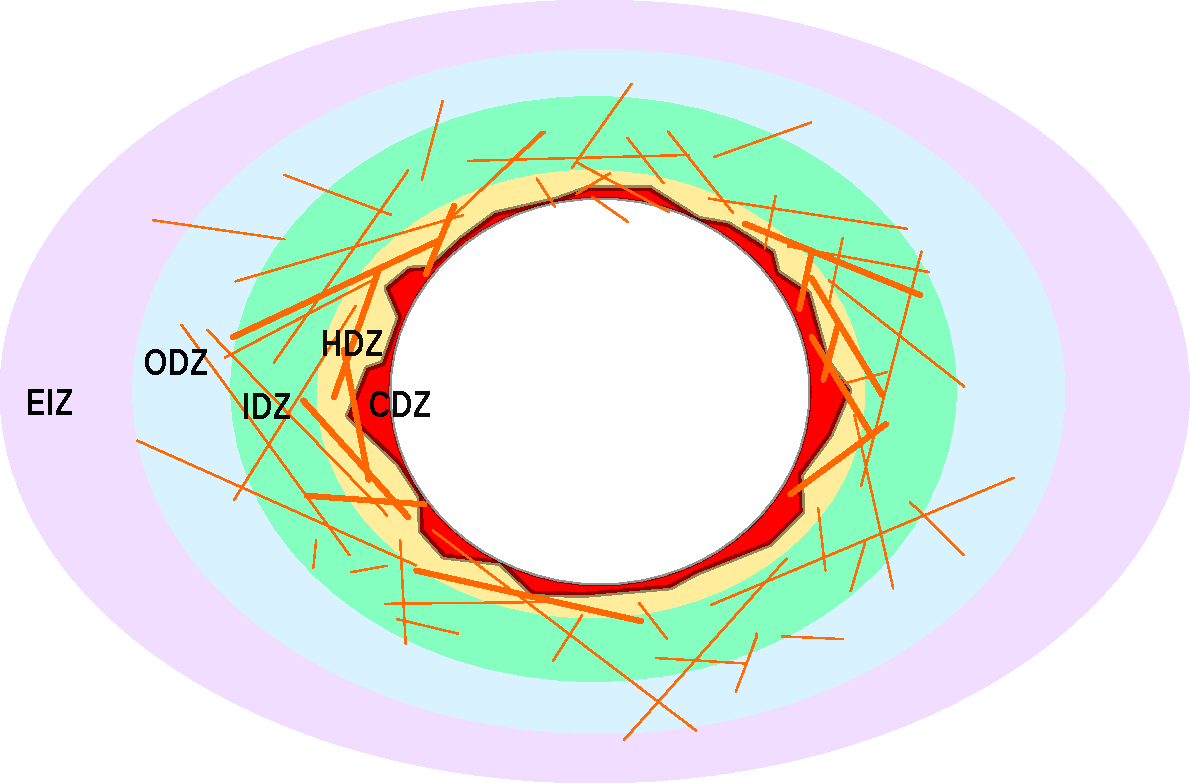
\includegraphics[width=\textwidth]{graphics/EDZ_structure.pdf}
    \caption{Označení zón s kvalitativně odlišnými změnami v důsledku vzniku díla.}
    \label{fig:edz_zones}
\end{figure}

Členění je závislé na rozdělění puklin na ``mikropukliny'' a ``makropukliny''
Všechny tyto zóny mohou mít zvýšenou hydraulickou vodivost oproti neporušené hornině. Pro EIZ nárůst vodivosti, díky preexistujícím poruchám a změnám porozity.

\subsection{Modely poškození}
Modely EDZ navržené v této sekci vychází zejména z obsáhlejší rešerše , přehledového článku \cite{Shahbazi2020a} a jejich citací.


V této sekci jsou shrnuty práce a modely vzniku EDZ zahrnující hydro-elastické modely, modely plasticity, pevnostní kritéria a modely poškození. Výsledkem těchto modelů může být rozsah jednotlivých zón, rozložení napětí a různé míry poškození.



TODO:
- otázka zda je difúze zanedbatelná při malých rychlostech
- zjistit řádově rychlosti na úrovni úložiště
- pro začátek bychom difúzi zanedbali

- klíčový parametr tenzor počátečního napětí
  lze měřit a lze získat 

- výpočet 
- tlak bentonitu 2,5 az 5 MPa, to je zhruba srovnatelne s hg tlakem v 500m cca 5MPa
- Grimsel v zule + teplo, pomala saturace, nebyla saturace ani po 18letech
- 

\subsection{Predikce vodivosti - geometrický přístup}
Dělení na podoblasti dle \cite{Perras2016}, lze založit buďto na 
Hosek-Brown kritériu \cite{}
\cite{Hajiabdolmajid2002}
Možnosti predikce:
\begin{enumerate}
    \item {\bf EIZ - elastický režim} Dokonale vratné malé i velké deformace, pouze změna porozity a tedy změna vodivosti dle Carman-Koženého.
    \item {\bf EDZ - plastický režim} Nevratné změny, vznik drobných poruch, které nelze rozlišit na modelech v měřítku průměru chodby, elementy cca do 1cm. 
    
    Lze použít empirické vztahy \cite{Rutqvist2009} závislosti na deformaci nebo napětí. Dále vztahy závislosti na Rock Mass Rating (z jader) \cite{Liu1999}. Případně jiné. 
    Asi použitelná první možnost, pokud se provede nějaká kalibrace pomocí vhodného měření in situ. \todo{další empirické nelineární vztahy mezi napětím a vodivostí, kalibrované pomocí 
    např. DFN modleu REV (zjednodušený víceškálový přístup).}
    \todo{Podrobněji popsat, uvést odkazy.}
    
    
    Lze uvažovat víceškálový model (snad možno zachytit vznik poruch do velikosti 1um). Na čtverci (1x1cm) uvažujeme náhodné pole mechanických parametrů (elastický tenzor a plastická kritéria). Plastická oblast detekována makro modelem, na ní provedena detailní analýza mikro výpočtem, aplikujeme příslušné pole deformace z makro modelu, v jednoduchém případě počítáme opět plastický model, případně na základě výsledků vygenerujeme nové pukliny a opakujeme výpočet. Následně určíme ekvivalentní tenzor vodivosti. Případně lze průměrovat přes více realizací, resp. lze získat populaci hodnot pro samplování v makro modelech transportu. 
    
    Zde by bylo výhodou, že parametry plastických modelů lze snad určit laboratorně na odvrtaných nepoškozených vzorcích.
    
    \item {\bf HDZ - makro poruchy, propojené} 
    Dle \cite{Perras2016} lze detekovat i tuto zónu plastickým modelem. Je otázkou zda ji je nutné uvažovat, jednak se předpokládá šetrný způsob ražby, ideálně pomocí TBM. Dále lze snad tuto zónu   
    
    Závislost vodivosti na deformaci (Kožený), dále závislost na napětí (Rutqvist), nutno fitovat empirické konstanty pomocí experimentu. 
\end{enumerate}


Hydraulická vodivost $K$ $[m/s]$ je vztažena k permeabilitě $\kappa$ $[m^2]$:
\[
    K =\frac{\kappa \rho g}{\nu}.
\]
pro tekutinu o hustotě $\rho$ $[kg\, m^{-3}]$ a hydrodynamické viskozitě $\nu$ $[s^-1]$.

{\bf Závislost permeability na geometrii.} Pro systémy paralelních nezávislých puklin odvozen kubický zákon: Snow (1965) \cite{Snow1965}:
\[
    \kappa=\frac{d^3}{12 D},
\] 
kde $d$ $[m]$ je rozevření puklin a $D$ $[m]$ je vzdálenost puklin. Pro složitější systémy puklin byly publikovány různé empirické homogenizace, e.g. \cite{Pouya2011}, další možností je použití více škálového modelu, kde je efektivní vodivost rozpukaného média vypočtena na základě mikro modelu. 
Různé homogenizační techniky pro ekvivalentní vodivost směsi materiálů jsou shrnuty v Renard 1997 \cite{Renard1997}.
Zde jsou populární DFN (Discrete fracture network) modely. Ovšem zde je opominutý významný příspěvek mikro puklin k celkové vodivosti, proto preferujeme použití continuum-fracture modelu.


Závislost vodivosti na porozitě je dána Carman-Koženého vztahem:

Vavro (2016) \cite{SURAO_50/2016}: Shrnutí zahraničních poznatků o vzniku a vývoji EDZ v krystalických horninách. Komplexní rešerše k tématům: definice EDZ, vliv EDZ na bezpečnost, mechanismy vzniku EDZ, metody charakterizace EDZ, přehled experimentálníc dat.

\begin{itemize}
    \item dělení EDZ, definice - pro model nepoužitelné
    \item možné pozitivní vlivy EDZ na bezpečnost \cite{Lanyon2011}: hydraulic cage, sorption surface on new fractures, ventilation of gasses, reduction of local transmissivity??
    \item Zdroje poškození:
    
\end{itemize}




\subsection{Rešerše - přehled souvisejících článků}
{\bf \cite{Shahbazi2020a}}\\
Přehledový článek o různých analytických a numerických modelech 
pro prdikci hydraulické vodivosti rozpukaného prostředí i na základě mechaniky. Z numerických přístupů 
jsou použity převážně DFN (discrete fracture networks) a DEM (distinct element method). 
TODO: projiít odkazy, hledání multiscale přístupu, jednoduchý model pro jemnou škálu s puklinami, 
efektivní parametry pro makro škálu

\noindent{\bf \cite{Blaheta2013}}\\
TH model pilíře v laboratoři \"Asp\"o se zahrnutím plasticity a modelů poškození. 
Kalibrace na některé měřené veličiny.



\noindent{\bf \cite{Perras2016}}\\
Použití DISL - damage initiatin and spalling pro predikci hloubky jednotlivých částí EDZ,
porovnání numerických modelů a empirických dat, fitování empirického vztahu pro relativní hloubku 
($r/R$) v závislosti na maximálním tečným napětím na stěně normalizovaném na CI (crack initiation napětí)
,$\sigma_{max} / \sigma_{CI}$. To je nelineární rozšíření vztahu navrženého v
\cite{Martin1999} a \cite{Diederichs2007}). 
DISL je založen na Hošek-Brownově kritériu.

\noindent{\bf \cite{Martin1999}}\\
Analýza hloubky poškození v závislosti na napětí a tvaru tunelu, krystalinika, založeno na Hošek-Brown.





\noindent{\bf \cite{Souley2001}}\\
Model poškození a model změny permeability, 
empirické, vazba na experimenty. Implementováno v SW FLAC3D (použito v projektu Hluboké horizonty).

\noindent{\bf \cite{Rutqvist2003}}\\
Přehled HM modelů pro rozpukanou horninu s různými konstitutivními 
vztahy pro explicitní popis vlastností puklin v závislosti ne tečném a normálovém napětí. 
Příklady aplikací a porovnání s měřeními.
Vztah mezi permeabilitou a "confining pressure" 
(pokles vodivosti s hloubkou. Jsou diskutovány vztahy mezi napětím resp. 
porozitou a permeabilitou. Matematický popis jevů na puklinách. Rozdíl mezi "apparent aperture" 
a "real apperture". 



{\bf \cite{Kelsall1984}}:\\
Základní článek zabývající se otázkou změny hydrulické vodivosti v EDZ. 
Odvozeno analytické řešení pro rozložení napětí v okolí ideální kruhové chodby. 
Změny v hydraulické vodivosti jsou dále odvozeny na základě kubického zákona. 
Na základě tohoto modelu predikují zvýšení vodivosti o jeden až dva řády pouze vlivem změny napětí. Změna alespoň o jeden řád nejvýše do vzdálenosti dvou průměrů od stěny chodby. Ražba střílením může dále zvýšit hydraulickou vodivost, avšak jen v blízkosti (cca. 0,3 m) stěny chodby.


{\bf \cite{Lisjak2014}}\\
Modelování vzniku puklin v EDZ pomocí \uv{hybrid finite discrete elements method},
přehled jiných numerických přístupů. 

{\bf  \cite{Barton1985}}\\
Measurement of fracture apperture and "real" apperture used in models.



\section{Inverzní úlohy a geofyzikální měření}
Jelikož cílem projektu je poskytnout predikci indikátorů bezpečnosti 
včetně charakterizace nejistot, je třeba standardní inverzní metody při zpracování geofyzikálních a jiných dat nahradit Bayesovskými inverzními metodami. Bayesovský přístup bude nejprve aplikován samostatně na vybrané druhy dat, která umožní nejlépe identifikovat parametry transportního modelu a modelu EDZ. V této sekci jsou shrnuty práce věnované experimentální charakterizaci EDZ s využitím různých metod.

S ohledem na výslednou permeabilitu zavedeme vlastní rozčlenění EDZ na základě mechanických dějů:
\begin{itemize}
    \item [Damage zone] - dochází k tvorbě nových makroskopických puklin, poškození
    \item [Plastic zone] - plastická (mikro trhliny)
    \item [Elasitic zone] - non-linear elasticity (fracture openning)
\end{itemize}
Není jasné co je v pracech myšleno pojmem "reverzibilní změny", jelikož i elasticky reverzibilní deformace jsou reálně irreverzibilní (nedojde k obnově původního napětí).



Změny v EDZ jsou HM proces a mhou tedy probíhat déle v závislosti na hydraulické vodivosti. Pro vodivost 1e-9 je čas transport na vzdálenost 1m při tlakovém spádu 1m cca 31 let. Reálné relaxační časy budou výrazně kratší, ale určitě v řádu dnů nebo měsíců. 

\section{Identifikace parametrů}
\label{sec:parameters}

Tato kapitola shrnuje měřící techniky, které mohou poskytnout přímou nebo nepřímou informaci 
o fyzikálních vlastnostech EDZ. Zejména nás zajímá charakterizace permeability, puklinových statistik a porozity. Ale i mechanické parametry: modul pružnosti, Poissonovo číslo, anisotropie elastického tensoru,  parametry plasticity ...
Převážně založeno na Vavro (2016) \cite{SURAO_50/2016} a doplněno o méně obvyklá měření.

{\bf MWD (Measure While Drilling)} \cite{JeroenvanEldert2018}

{\bf GPR (Ground Penetrating Radar)} 

{\bf ERT (Electrical resistence tomography)}


{\bf Seismicity}

{\bf  Borehole Core Drilling and Logging} \cite{Lanyon2011}

{\bf Mapping of the Excavation Surfaces} \cite{Lanyon2011}

{\bf  Resin Injection and Overcoring} \cite{Lanyon2011}

{\bf  Sonic and Ultrasonic Measurements} \cite{Lanyon2011}
{\bf  Acoustic Emission} \cite{Lanyon2011}

{\bf  Resistivity/Geo-electrical Measurements} \cite{Lanyon2011}

{\bf  Radar Measurements} \cite{Lanyon2011}

{\bf  Hydraulic Characterization} \cite{Lanyon2011}

{\bf  Geomechanical Characterization} \cite{Lanyon2011}

{\bf  Geochemical Characterization} \cite{Lanyon2011}

{\bf MVP - microvelocity probe} \cite{Rutqvist2009} 
{\bf SEPPI - a permeability measurement} \cite{Rutqvist2009} 


\subsection{Rešerše prací}

{\bf Říha et al. (2019)} Task G, TAS04: Dostupná data: 
\begin{itemize}
    \item Geometrie tunelu, mračno bodů.
    \item Počáteční a koncový bod vrtů (celkem 15 z toho 3 vtláčecí a 4 měřící).
    \item Otevřené zóny vrtů (10-20cm, 20-40cm, 40-60cm).
    \item Pukliny odečtené na povrchu tunelu.
    \item Průměrné charakteristiky horniny.
    \item GPR data, identifikované pukliny do hloubky 40cm.
    \item DFN - stochasticaly generated (not clear for which statistical parameters)
    \item Odhadované charakteristiky EDZ jako kontinua.
    \item Overall pressure and stress gradiends in the domain.
\end{itemize}

{\bf Aoyagi and Ishii al. (2018)} \cite{Aoyagi2018}: horní odhad hydraulické vodivosti v EDZ (laboratoř Horonobe, Japonsko) na základě MSI (Mean Stress Index). Model porovnán s měřením z různých metod: průměrné charakteristiky horniny z různých měření, vizuální identifikace puklin v konkrétních vrtech (rozevření nad 0,1 mm), klasifikace puklin v jádrech, měření mechanických posunutí v chodbě, tlakové zkoušky.

{\bf Armand et al. (2014)} \cite{Armand2014}: Charakterizace indukované sítě puklin v EDZ v laboratoři URL (Bure, Francie). Použité metody: 3d sken jader, analýza puklin na jádrech, seismická měření, hydraulické testy a injektáž pryskyřice ve vrtech. 

{\bf Bláha et al. (2017)} \cite{SURAO_184/2014}: přehled geofyzikálních měření na PVP Bukov.
Podrobná zpráva o ERT a seismických měřeních na PVP Bukov, interpretace s předpokládanou hranicí zóny poškození, resp. zóny ovlivnění.  

{\bf Staš a Bláha (2019)} \cite{SURAO_351/2019}: Vznik a monitoring EDZ při výstavbě PVP Bukov.
Podrobná zpráva o dlouhodobém monitorování napětí během vzniku EDZ, identifikace původního napětí v hornině. Celkově rozporuplné výsledky v důsledku velké heterogenity horniny a lokálnímu charakteru metody. Shrnutí ERT a seismických měření, interpretace s předpokládanou hranicí EDZ.  

{\bf Eldert (2018)} \cite{JeroenvanEldert2018}: Charakterizace blast damage for the DaB (drill and blast) method. Využití MWD pro predikci EDZ.


\bibliography{zprava.bib}


\pagebreak


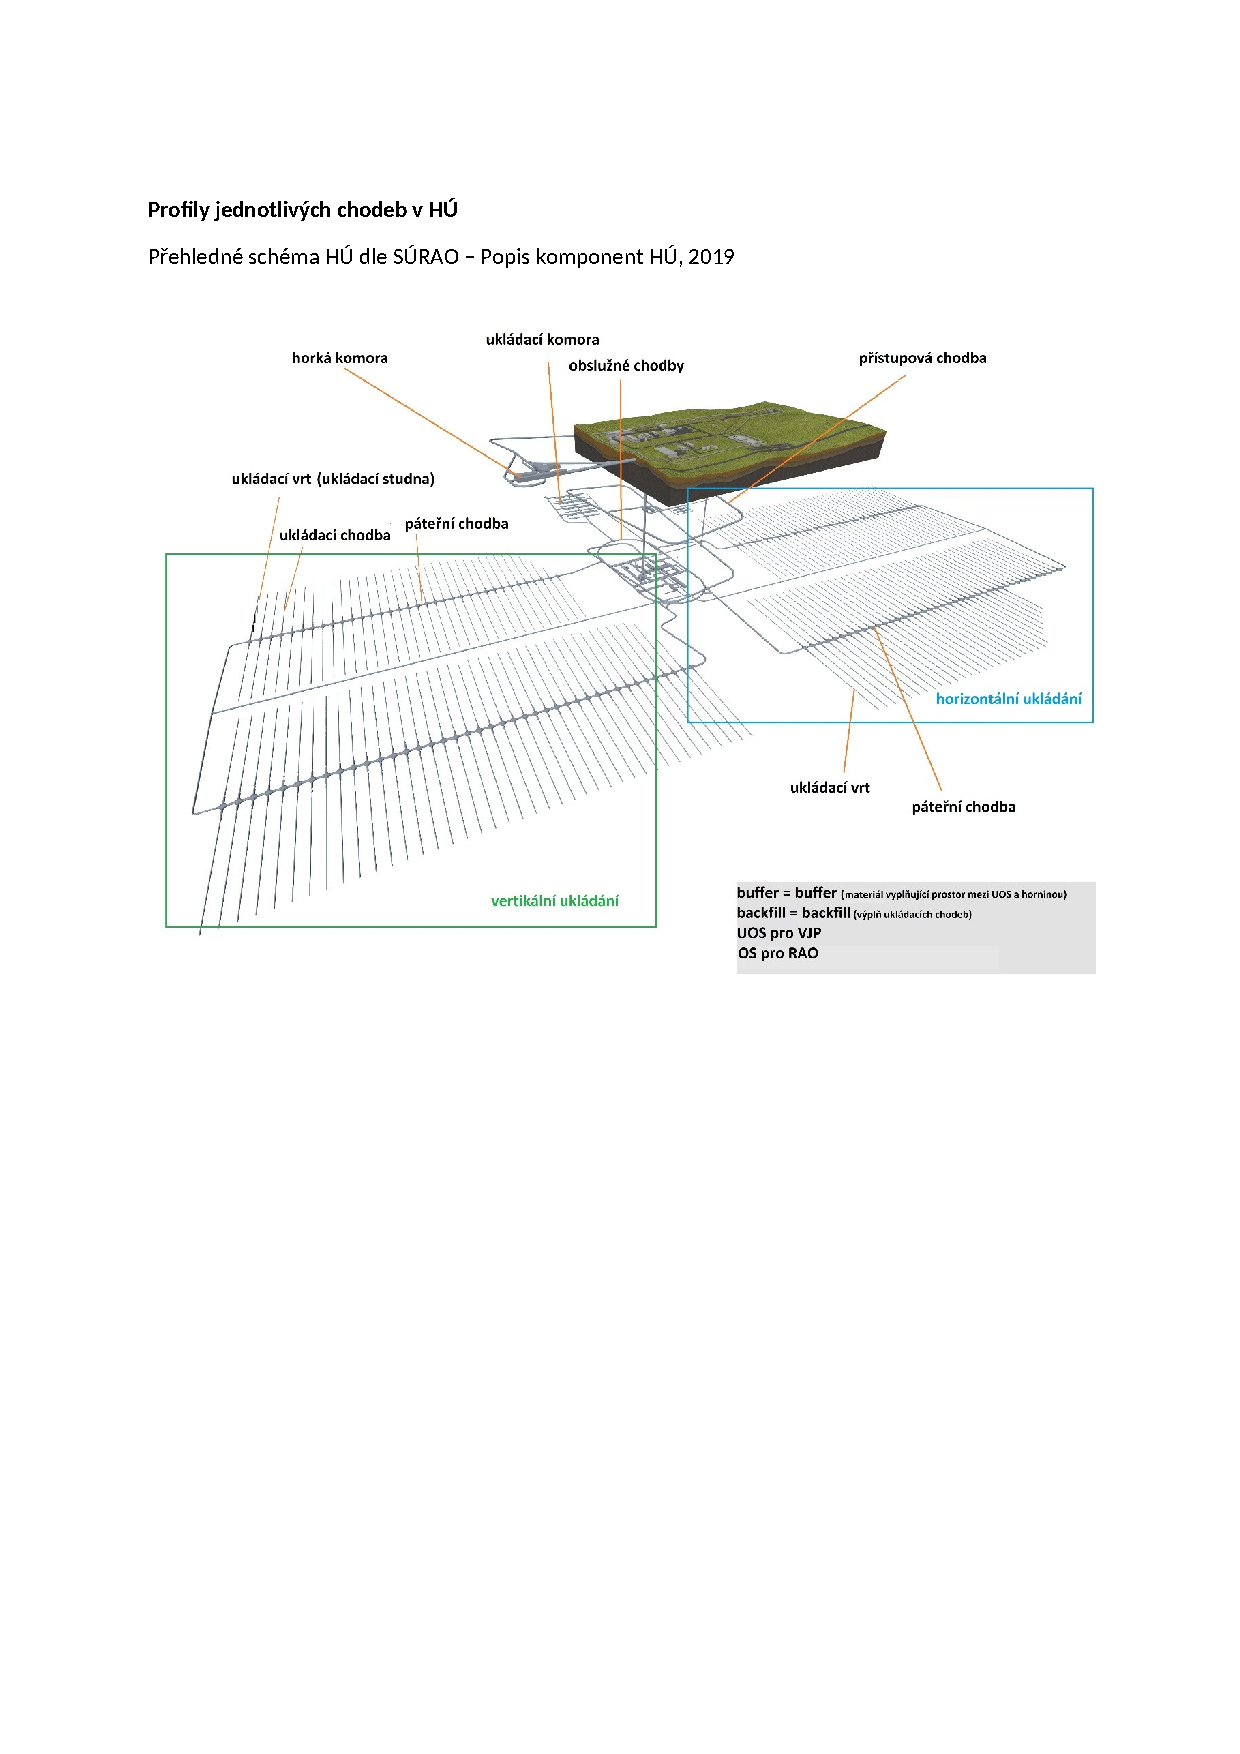
\includepdf[scale=0.99, offset=0 -3cm, page={1},
pagecommand=\section*{Dodatek A - Geometrie HÚ dle SÚRAO}]{Geometrie_HU.pdf}

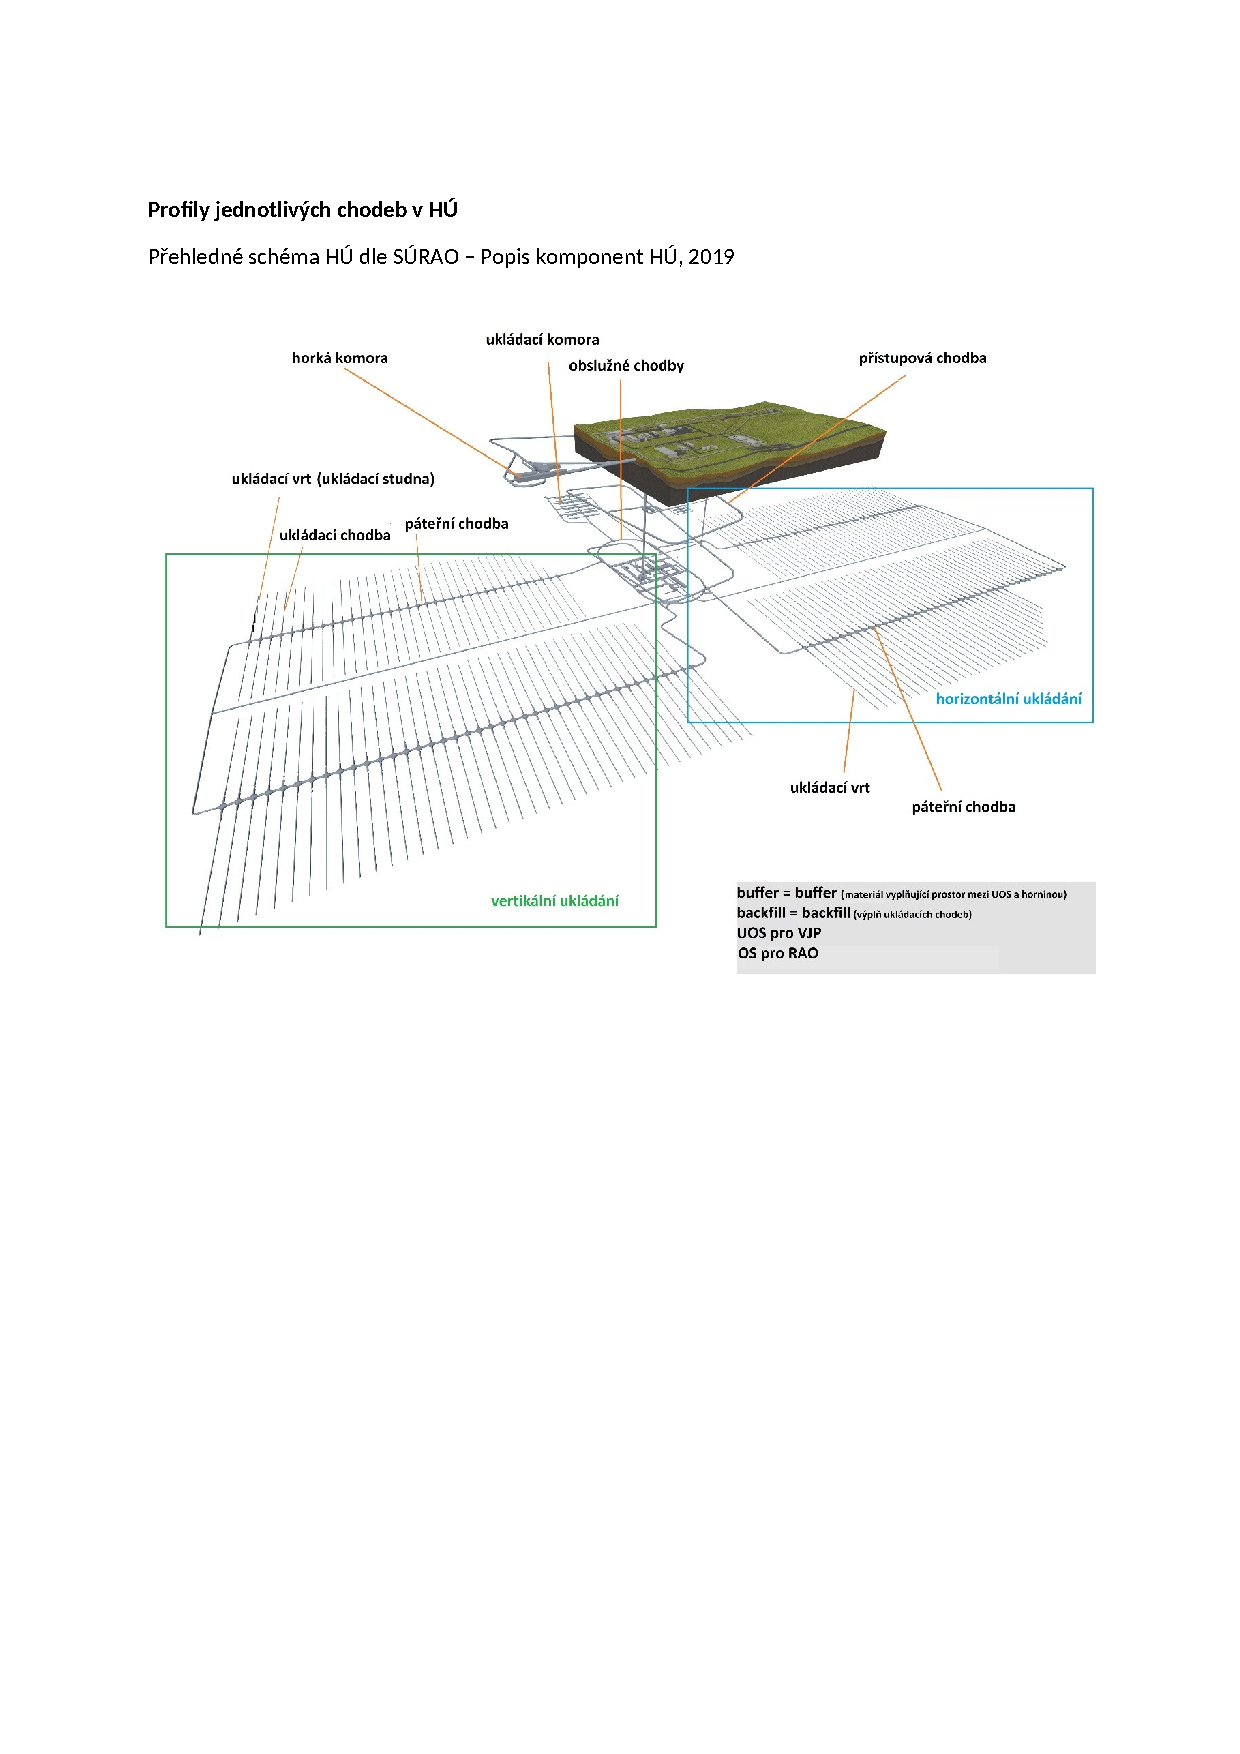
\includepdf[scale=0.99, offset=0 -3cm, page={2,3}]{Geometrie_HU.pdf}

\section*{Dodatek B - odvození řešení rovnice advekce-difúze}
Hledejme nejprve řešení rovnice bez rozpadů na pravé straně:
\begin{equation}
    \label{eq:no_decay_ad}
    R\prtl_t c + v \prtl_x c - d \prtl^2_x c = 0
\end{equation}

pro neznámou koncentraci $c(t, x)$ pro časy $t>0$ a na oblasti $x>0$ s počáteční podmínkou $c(0, x) = 0$ a
okrajovými podmínkami:
\[
    \prtl_t c(t, \infty) = 0,
\]
\[
    c(t, 0) = c_0(t),
\]
kde $c_0 \in C^\infty$.

Analytická řešení a aproximativní řešení uvedené rovnice pro různé druhy počátečních
a okrajových podmínek lze nalézt v \cite{Genuchten1982} (str. 9). 
Speciálně pro případ skokové okrajové podmínky:
\begin{equation}
    \label{eq:jump_bc}
    c_0(t) = \left\{\begin{array}{ll}
         0 & 0 < t < t_0 \\
         1   & t_0 < t
    \end{array}\right. 
\end{equation}
má rovnice řešení:
\begin{equation}
    \label{eq:jump_sol}
    \tilde c(t, x) = 
    \left\{\begin{array}{ll}
         0                     & 0 < t < t_0 \\
         A(t,x)   & t_0 < t,
    \end{array}\right. 
\end{equation}

kde
\[
    A(t,x) = \frac12 \mathrm{erfc}\Big(\frac{ax-bt}{\sqrt t}\Big)
    + \frac12 e^{cx}\mathrm{erfc}\Big(\frac{ax+bt}{\sqrt t}\Big),
\]
\[
    a = \frac{R}{2\sqrt{dR}},\quad 
    b=\frac{v}{2\sqrt{dR}},\quad 
    c=\frac{v}{d}.
\]

Řešení pro obecný průběh okrajové podmínky $c(t,0) = c_0(t)$ lze napsat v konvolučním tvaru:
\[
    c(t,x) = \int_0^t c_0(s) g(t - s, x) ds,
\]

kde jádro $g(t - s, x)$ je řešením rovnice pro okrajovou podmínku $c_0(t) = \delta(t - s)$. 
Tato okrajová podmínka je formálně derivací jednotkového skoku \eqref{eq:jump_bc}. 
Proto jádro bude derivací odpovídajícího řešení:
\[
    g(t, x) = \prtl_t A(t, x) = 
    \frac{1}{2\sqrt{\pi}} 
    e^{-\big( \frac{ax-bt}{\sqrt{t}}\big)^2}
    \Big[ ax t^{-\frac32} + b t^{-\frac12}\Big]
    + \frac{e^{cx}}{2\sqrt{\pi}}  
    e^{-\big( \frac{ax+bt}{\sqrt{t}}\big)^2}
    \Big[ ax t^{-\frac32} - b t^{-\frac12}\Big].
\]
Tento tvar by měl být použitelný i pro nuerický výpočet.


Řešení rovnice s rozpadovým členem na pravé straně
\[
 R\prtl_t c + v \prtl_x c - d \prtl^2_x c = - \lambda c
\]
pro stejné okrajové a počáteční podmínky pak nalezneme ve tvaru:
\[
    c(t,x) = U(t,x) e^{-\lambda t},
\]
kde $U(t,x)$ řešením rovnice bez rozpadového členu \eqref{eq:no_decay_ad}, ovšem s okrajovou podmínkou
\[
    \tilde{c}_0(t) = c_0(t) e^{\lambda t}.
\]


% Rovnici vydělíme $R$, označíme
% \[
%     v_r = v/R,\quad d_r = d/R,\quad \lambda_r = \lambda/R.
% \]
% a provedeme transformaci:
% \[
%     c(t, x) = g(t, z),\quad z = \frac{x - v_r t}{\sqrt{d_r}}.
% \]
% Obdržíme rovnici:
% \[
%     \prtl_t g -  \Delta g = - \lambda_r g
% \]
% pro $t>0$, $z > - \frac{v_r t}{\sqrt{d_r}}$, $g(0, z) = 0$, $g(t, \frac{- v_r t}{\sqrt{d_r}}) = c_0(t)$.

% Její řešení má tvar:
% \[
%   g(t,z) = G(t,z) e^{-\lambda_r t}
% \]
% kde $G(t, z)$ je řešení homogenní rovnice:
% \[
%     \prtl_t G -  \Delta G = 0
% \]
% s okrajovou podmínkou $G(t, \frac{- v_r t}{d_r}) = c_0(t) e^{\lambda_r t}$.

% Jádro $\phi(t, z)$ pro 


% \begin{equation}
%     g(t, z) = (4\pi t)^{-\frac12} e^{\frac{-z^2}{4t}} e^{-\lambda_r t},\quad
%     ,
% \end{equation}
% kde jsme označili




\end{document}
